% This LaTeX document needs to be compiled with XeLaTeX.
\documentclass[10pt]{article}
\usepackage[utf8]{inputenc}
\usepackage{amsmath}
\usepackage{amsfonts}
\usepackage{amssymb}
\usepackage[version=4]{mhchem}
\usepackage{stmaryrd}
\usepackage{graphicx}
\usepackage[export]{adjustbox}
\graphicspath{ {./images/} }
\usepackage{bbold}
\usepackage[fallback]{xeCJK}
\usepackage{polyglossia}
\usepackage{fontspec}
\IfFontExistsTF{Noto Serif CJK TC}
{\setCJKmainfont{Noto Serif CJK TC}}
{\IfFontExistsTF{STSong}
  {\setCJKmainfont{STSong}}
  {\IfFontExistsTF{Droid Sans Fallback}
    {\setCJKmainfont{Droid Sans Fallback}}
    {\setCJKmainfont{SimSun}}
}}

\setmainlanguage{english}
\IfFontExistsTF{CMU Serif}
{\setmainfont{CMU Serif}}
{\IfFontExistsTF{DejaVu Sans}
  {\setmainfont{DejaVu Sans}}
  {\setmainfont{Georgia}}
}

\begin{document}
\section*{Introduction to binth \& death Markov processes}
We discuss here a simple class of Markov processes, those that have a set of states that can be labeled with integers. We start from an even simpler discrete Morkor process, the binth and deoth processes which occur in mony applications. Then we will deduce results to more general coses.\\
We otact from a rituation that is very similar to the zondom wolk. We assume discrete times $t=0, \Delta t, 2 \Delta t, \ldots$ discrete states $x=0, \pm 1, \pm 2 \ldots$ and that jumps are allowed only between nearest neighbors, i.e. from $n$ to $n \pm 1$. For $\Delta t \ll 1$ we call $b_{n} \geqslant 0$ the birth wate, i.e., $b_{n} \Delta t$ is the prob. to jump to $n+1$ at time $t+\Delta t$, given that at time $t$ the state was $n$. (notice that $b_{n}$ daes not depend on time, thangh it cauld in principle. If it does not, we say that the process is homogeneous). Analogously, $d_{n} \geqslant 0$ is the death rate, i.e. $d_{n} \Delta t$ is the prob. to jump to $n-1$ at time $t+\Delta t$, given that at time $t$ the strate was $n$.\\
We want to calculate the prob. $p(n, t+\Delta t)$ (the propagotor).\\
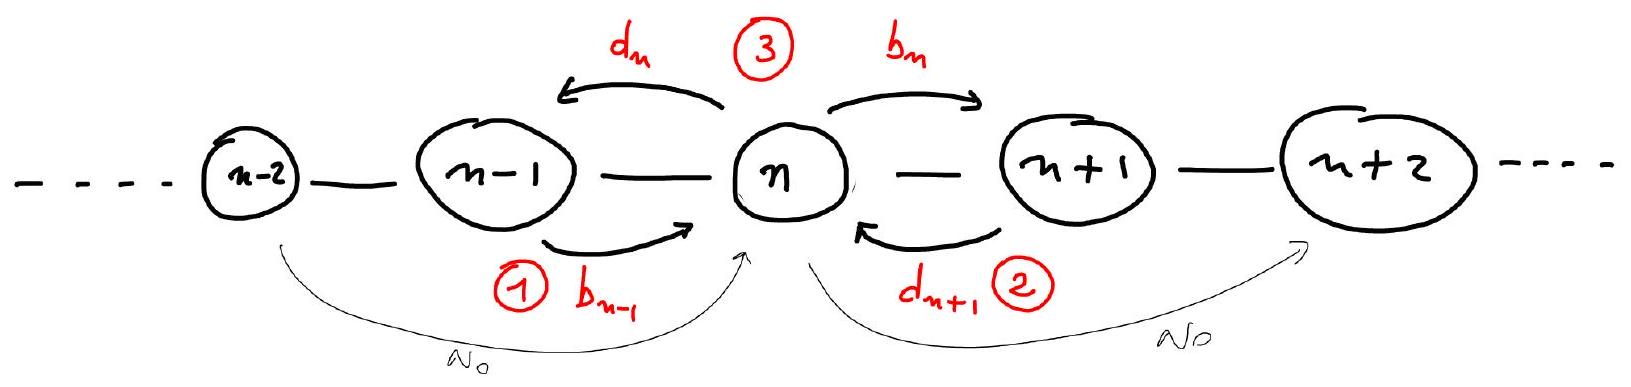
\includegraphics[max width=\textwidth, center]{2025_10_17_b1062645fdca57c84af1g-01}


\begin{equation*}
p(n, t+\Delta t)=b_{n-1} \Delta t p(n-1, t)+d_{n+1} \Delta t p(n+1, t)+\left[1-\left(b_{n}+d_{n}\right) \Delta t\right] p(n, t) \tag{1}
\end{equation*}


By Taylor exponsions and then taking the limit $\Delta t \rightarrow 0$ we get\\
(1) $\quad \frac{\partial p_{n}}{\partial t}=b_{n-1} p_{n-1}(t)+d_{n+1} p_{m+1}(t)-\left(b_{n}+d_{n}\right) p_{n}(t)$

This is called the moster equation of the binth-deoth process or generation-riconlaination process.

A few observations:

\begin{enumerate}
  \item The M.E. is a gain-loss equation for the probabilities $p_{n}$;
  \item We have to equip ey. (1) with imitial conditions. If We start with $P_{n, n_{0}}\left(t_{0}\right)=\delta_{m_{1} m_{0}}$, then the M.E. is the equation of the propogator of the Mackov process, that is
\end{enumerate}

$$
P_{n}(t) \equiv P\left(n, t \mid n_{0} t_{0}\right)
$$

So ane con show (exercize) that $p_{n}(t)$ satisfies the ChapmanKolmogozov ep. in its obfferential form. More fallows on this.\\
3) We con introduce boundary conditions as well. For instance, if $N$ is a reflecting boundary,\\
(2)\\
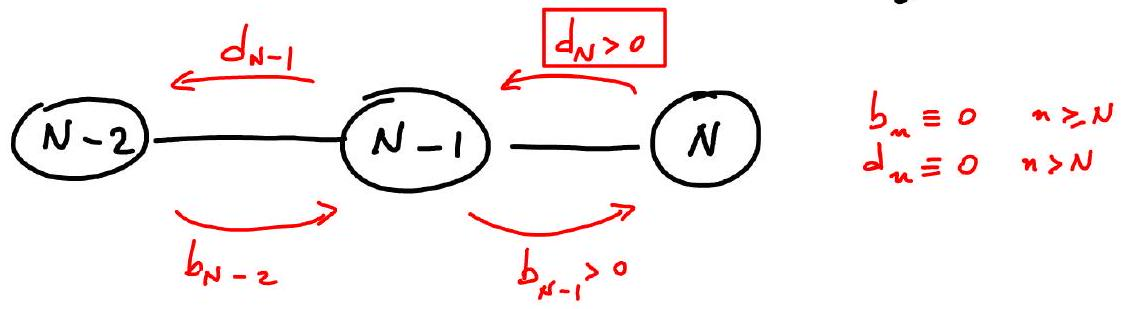
\includegraphics[max width=\textwidth, center]{2025_10_17_b1062645fdca57c84af1g-02}\\
then $b_{n} \equiv 0 \forall n \geqslant N, d_{n} \equiv 0 \forall n>N \quad\left(\right.$ for $n<N, b_{n}$ and $d_{n}$ ore $\left.\geqslant 0\right)$ therefore if the state $N$ is reached, it can be left from one side only. $N$ is a reflecting state.

If $N$ is ar absolsing boundry,\\
(3)\\
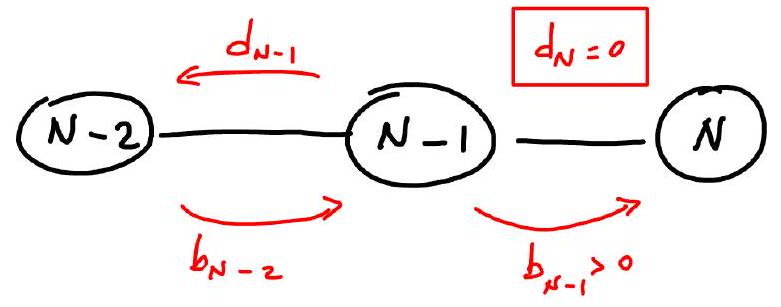
\includegraphics[max width=\textwidth, center]{2025_10_17_b1062645fdca57c84af1g-03}\\
here $d_{N}=0$ which is important, because when the state $N$ is reached, it con no longer be left. We say that $N$ is an absorbing state.

\section*{Warning:}
Because of the b.c. We have to be coreful with ep. (1) as it holds only when the boundory states are not hit, otherwise it must be changed.\\
4) Notice that ep. (1) is limeor and deterministic; indeed we con define a matrix $\mathbb{W}$ whose entries are\\
(42) $\mathbb{W}_{m m^{\prime}}=d_{m^{\prime}} \delta_{m, m^{\prime}-1}+b_{m^{\prime}} \delta_{m, m^{\prime}+1}-\left(d_{m}+b_{m}\right) \delta_{m, n^{\prime}}$

So, if we introduce the vector notation $[\vec{p}(t)]_{n} \equiv p_{n}(t)$ we con write ef. (1) as\\
(4b) $\quad\left\{\begin{array}{l}\dot{\vec{P}}(t)=\mathbb{W} \vec{P} \\ \vec{P}(0)=\vec{P}_{0}\end{array}\right.$\\
and formally the solution reads $\vec{P}(t)=e^{W / t} \vec{P}_{0}$.\\
The moster equation defined in ep. (4b) holds in general for a continuous time, discrete Morkov process as long as $\mathbb{W}$ sotisfies the following properties:

\begin{enumerate}
  \item $W_{n x^{\prime}} \geqslant 0$ for $n \neq n^{\prime}$
  \item $\sum_{m} \mid \mathbb{W}_{m n^{\prime}}=0$ for each $n^{\prime}$ (no abs. bound.)
\end{enumerate}

The equations for the mean and the variance Frome op. (1) One con simply desive the eps. for the fine evolution of the mean and the verionce. We first multiply of. (1) by $x$ and sum over $x$ : $\langle n\rangle \equiv \sum_{-\infty}^{+\infty} x^{n} p_{n}(t)$

$$
\begin{aligned}
\frac{d}{d t}\langle n\rangle & =\sum_{-\infty}^{+\infty}\left(n b_{n-1} p_{n-1}-n b_{n} p_{n}+n d_{n+1} p_{n+1}-n d_{n} p_{n}\right) \\
& =\sum_{n}\left[(n+1) b_{n} p_{n}-n b_{n} p_{n}+(n-1) d_{n} p_{n}-n d_{n} p_{n}\right] \\
& =\sum_{n}\left(b_{n}-d_{n}\right) p_{n}
\end{aligned}
$$

(5)

$$
\begin{array}{ll}
\frac{d}{d t}\langle n\rangle=\left\langle b_{n}\right\rangle-\left\langle d_{n}\right\rangle & \left\langle b_{n}\right\rangle \equiv \sum_{n} b_{n} p_{n} \\
& \left\langle d_{n}\right\rangle \equiv \ldots
\end{array}
$$

with some initial conditions. Notice that this equation has to be opuipped with different equations if there is an absorbing or reflecting b.c. Can you find them?

For the evolution of the verionce we have to desive an equation for the second moment $\left\langle n^{2}\right\rangle$. We first multiply ep. (1) by $n^{2}$ and then sum over $n$ :

$$
\begin{aligned}
\frac{d}{d t}\left\langle n^{2}\right\rangle & =\sum_{-\infty}^{+\infty} n n^{2}\left(b_{m-1} p_{m-1}+\cdots\right)= \\
& =\sum_{m}\left((n+1)^{2}-n^{2}\right) b_{m} p_{m}+\sum_{m}\left[(n-1)^{2}-n^{2}\right] d_{m} p_{m} \\
& =\sum_{m}(2 n+1) b_{m} p_{m}+\sum_{m}(-2 n+1) d_{m} p_{m} \\
& =2 \sum_{m} n\left(b_{m}-d_{m}\right) p_{m}+\sum_{m}\left(b_{m}+d_{m}\right) p_{m}
\end{aligned}
$$

Thus\\
(6) $\frac{d}{d t}\left\langle m^{2}\right\rangle=2\left\langle n\left(b_{n}-d_{n}\right)\right\rangle+\left\langle b_{n}+d_{n}\right\rangle$

The equilibrium distribution\\
For binth and deoth procen it is possible to colculate the equilibrium distribution of ef. (1) in general. This is not possible for more complicated discrete Marker processes.\\
We will colulate the distribution for a $b / d$ process defined between O (2.b.c.) and $\infty$.\\
We con define a stationary flux from $n-1$ to $n$ :\\
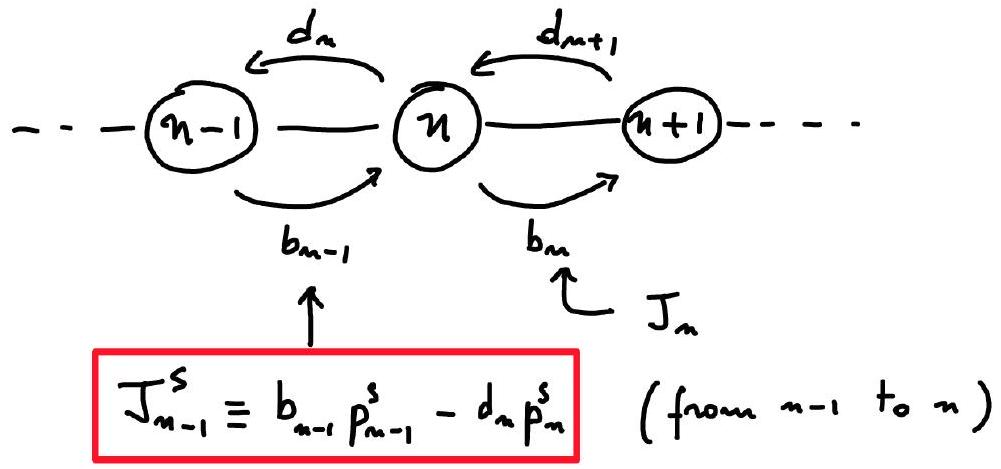
\includegraphics[max width=\textwidth, center]{2025_10_17_b1062645fdca57c84af1g-05}

From ep. (1) we get then

$$
D=\underbrace{b_{n-1} p_{n-1}^{s}-d_{n} p_{n}^{3}}_{J_{n-1}}+\underbrace{d_{n+1} p_{n+1}^{s}-b_{n} p_{n}^{s}}_{-J_{n}}
$$

hence $J_{m}=J_{m-1}=\ldots=J_{0}-b_{-1} p_{-1}^{3}-d_{0} p_{0}^{3}=0 =0 \quad=0$ Truff.b.c. at $m=0$\\
then

$$
\begin{gathered}
J_{n}=b_{n-1} p_{n-1}^{s}-d_{n} p_{n}^{s}=0 \Rightarrow b_{n-1} p_{n-1}^{s}=d_{n} p_{n}^{s} \quad \text { DETAILED } \\
\text { BALANCE } \\
p_{n}^{s}=\frac{b_{n-1}}{d_{n}} p_{n-1}^{s}=\frac{b_{n-1}}{d_{n}} \frac{b_{n-2}}{d_{n-1}} p_{n-2}^{s}=\ldots \Rightarrow
\end{gathered}
$$

(7) $\quad p_{m}^{s}=\prod_{1}^{n} \frac{b_{i-1}}{d_{i}} p_{0}^{s} \quad$ for $n=1,2, \ldots$\\
becouse of normolizetion, $\left(p_{0}^{s}\right)^{-1}=1+\sum_{1}^{\infty} \prod_{i}^{\infty} \frac{b_{i-1}}{d_{i}}$; $p_{i}^{s}$ exists if $p_{0}^{s}<\infty$. The some approach can be used for a finite number of states $n=1, \ldots, N$.

\section*{Simple yet important birth \& death processes}
Poisson process\\
This procen is defined by the sotes $b_{n}=\lambda, d_{n}=0$, where $n=0,1, \ldots$ So the $M-E$. is\\
(8) $\quad\left\{\begin{array}{l}\dot{p}_{m}=\lambda\left(p_{m-1}-p_{m}\right) \\ p_{m}(0)=\delta_{m, 0}\end{array}\right.$

Ex: show that the mean sotisfies the eq. $\frac{d}{d t}\langle u\rangle=\lambda$ and so $\langle n(t)\rangle=n_{0}+\lambda t$ if $p_{n}(0)=\delta_{n, n}$ 。

We solve op. (8) with the method of the generating function:

$$
g(z, t) \equiv \sum_{0}^{\infty} z^{n} p_{n}(t)
$$

So from ep. (8) we get an ef. for $g$ :\\
(9) $\quad\left\{\begin{array}{l}\frac{\partial}{\partial t} g(z, t)=\lambda(z-1) g(z, t) \quad\left(g(1, t)=\sum_{n} p_{n}(t)=1\right) \\ g(z, 0)=\sum_{n} z^{n} \delta_{n, 0}=1\end{array}\right.$

The solution of (3) is then


\begin{equation*}
g(z, t)=e^{\lambda(z-1) t}=e^{-\lambda t} \overbrace{\sum_{0}^{\infty} \frac{(\lambda t)^{n}}{n!} z^{n}}^{e^{\lambda z}}=\sum_{0=n}^{\infty} p_{n}(t) z^{n} \tag{8}
\end{equation*}


hence\\
(10) $p_{n}(t)=e^{-\lambda t} \frac{(\lambda t)^{n}}{n!}$

Show that $\operatorname{var}(n(t))=\lambda t$.

Radioactive decay\\
Unitially the rystem consists of $N_{0}$ sodioactive porticles which decay at sate $\gamma$. Therefore, if at time $t$ there are $n$ surviving perticles, then in the following $\Delta t$ time the probability of one decay is $\gamma n \Delta t$ and more thon one decay is $\sigma(\Delta t)$. Thus $d_{n}=\gamma_{n}$ and $b_{n}=0$ and the M.E. is

$$
\left\{\begin{array}{l}
\dot{p}_{n}=\gamma(n+1) p_{n+1}(t)-\gamma m p_{n}(t) \quad n=0,1 \ldots N_{0}-1 \quad \text { a.b.c. at } n=0 . \\
\dot{p}_{N_{0}}=-\gamma N_{0} p_{N_{0}}(t) \\
p_{n}(0)=\delta_{n, N_{0}}
\end{array}\right.
$$

Ex: show that $\frac{d}{d t}\langle n\rangle=-\gamma\langle n\rangle$, so $\langle n(t)\rangle=N_{0} e^{-\gamma t}$.\\
With the generating function $g(z, t)=\sum_{0}^{N_{0}} z^{n} p_{n}(t)$ we get

$$
\text { (11) } \quad \frac{\partial g(z, t)}{\partial t}=\gamma(1-z) \frac{\partial}{\partial z} g(z, t) \quad \begin{aligned}
& g(1, t)=1 \\
& g(z, 0)=z^{N}
\end{aligned}
$$

Notice that $h\left(z_{1} t\right)=\varepsilon(t)(1-z)+1$ leads to $\varepsilon=-\gamma \varepsilon$, namely $\varepsilon(t)=\varepsilon_{0} e^{-\gamma t}$, so $h(1, t)=1$, but $h(z, 0)=\varepsilon_{0}(1-z)+1 \neq z^{N_{0}}$. However, take $g$ as a function of $h$, i.c. $g(z, t)=f(h(z, t))$, we get from (11)

$$
\frac{\partial g}{\partial t}=\frac{d f}{d h} \frac{\partial h}{\partial t} \quad, \quad \frac{\partial g}{\partial z}=\frac{d f}{d h} \frac{\partial h}{\partial z}
$$

and $\frac{d f}{d h}$ simplifies, because it occurs on both sides of ey. (11). We con then use $f$ to satisfy the i.c.: $f(a)=a^{N_{0}}$ does the job. We take $g=\left(\varepsilon_{0} e^{-\gamma t}(1-z)+1\right)^{N_{0}}$ where $\varepsilon_{0}=-1$. Eventually, the sol, is\\
(12) $g(z, t)=\left(e^{-\gamma^{t}(z-1)+1}\right)^{N_{0}}$

We have now to invect this relation to get $p_{n}(t)$\\
$g(z, t)=\left(e^{-\gamma t} z+\left(1-e^{-\gamma t}\right)\right)^{N_{0}}=\sum_{0}^{N_{0}}\binom{N_{0}}{m}\left(1-e^{-\gamma t}\right)^{N_{0}-n} e^{-n \gamma t} z^{n}$\\
which gives\\
(13) $\quad p_{n}(t)=\binom{N_{0}}{n} e^{-n \gamma t}\left(1-e^{-\gamma t}\right)^{N_{0}-n}$

We con interpret this ep. in this way: $e^{-x \gamma t}$ is the prob. that $n$ particles have survived (i.e., not decayed yet) by time $t,\left(1-e^{-\gamma t}\right)^{N_{0}-n}$ is the prob. that $N_{0}-n$ porticles have decayed by time $t$. We also need the factor $\binom{N_{0}}{n}$ because the specific identity of the porticles is not important, then there ore $\binom{N_{0}}{n}$ Ways to select $n$ surviving particles out of $N_{0}$.

\section*{Furry process}
A cosmic electron enters an absorbing material (like lead...) and branches into multiple particles (an electron may emit a photon which moy then preduce an $e^{+}-e^{-}$poir). So a coscode of secondory poiticles is produced which generotes a shower of final porticles. This process can be deserved by a $b$ \& $d$ procen where $b_{n}=\gamma_{n}$ and $d_{n}=0, n=1,2, \ldots$\\
The M.E. is then

$$
\left\{\begin{array}{l}
\dot{p}_{n}=\gamma(n-1) p_{n-1}-\gamma n p_{n} \\
p_{n}(0)=\delta_{n, 1}
\end{array}\right.
$$

Show as before that

$$
\begin{aligned}
& \langle n(t)\rangle=e^{\gamma t} \\
& \operatorname{Var}(n(t))=e^{\gamma t}\left(e^{\gamma t}-1\right)
\end{aligned}
$$

Finally:\\
(14) $\quad p_{n}(t)=e^{-\gamma t}\left(1-e^{-\gamma t}\right)^{n-1}$ try to interpet the vesult.

\section*{The contect procen}
Let us assume that a population of $N$ individuals can be devided into two cotegories according to whether they are infected on not (but are susceptible any way). If an indiv. has not yet cought the infection, may catch it from any of of the $n$ infected ones (uniformly at random).\\
We con write down the trousition rote from $n$ to $n+1$ infected individuals; if the number of infected ind. increases by one, then one healthy ind. must get in conctact with an infected one:

\begin{enumerate}
  \item finst, we have to pick one healthy indiv.
\end{enumerate}

$$
b_{n}=\tilde{\beta} \frac{N-n}{N} \frac{n}{N-1}=\frac{\beta}{N} n(N-n)
$$

\begin{enumerate}
  \setcounter{enumi}{1}
  \item second, the healthy ind. have to encounter an infected one.
\end{enumerate}

We then assume that an infected individual recovers at rote $\gamma$. then the trousition rote from state $n$ to $n-1$ is $d_{n}=\gamma n$. Notice that $b_{0}=0=d_{0}$ ( $n=0$ is an assorbing state) and $b_{N}=0, d_{N} \neq 0 \quad(n=N$ is a reflecting state $)$ and we have to set $d_{N+1}=0$.\\
Notice that the zotes $b_{n}$ and $d_{n}$ con be written as a function of $x=\frac{N}{N}: b_{x}=N \beta \times(1-x), d_{x}=N \gamma x$.\\
As $N$ becomes large, the variations in $n$ become surall and so one hopes to describe $x$ as a continuous variable. Making this limit rigorous is tricky (Kurtz's theorem), but one con anywoy guess the limiting guation. the important assumption is the existence of a typical scale of the system (in this cose $N$ ) and that the perameters (here $\beta$ and $\gamma$ ) scale appropriately with $N$.

The master equation has a form\\
(15) $\quad \dot{q}_{n}(\epsilon)=b_{\frac{n-1}{N}} q_{n-1}+d_{\frac{n+1}{N}} q_{n+1}-\left(b_{\frac{n}{N}}+d_{\frac{n}{N}}\right) q_{n}$

In the continuous limit $q_{u}(t)$ becomes a $P D F$ of $x, s_{0}$ we write

$$
q_{n}(t)=\frac{1}{N} p(x, t) \quad \text { for lorge } N
$$

So eq. (15) becomes\\
(16)\\
$\dot{p}(x, t)=b_{x-\frac{1}{N}} p\left(x-\frac{1}{N}, t\right)+d_{x+\frac{1}{N}} p\left(x+\frac{1}{N}, t\right)-\left(b_{x}+d_{x}\right) p(x, t)$

As $\frac{1}{N}$ is surall, we con Taylar expand $\varphi$. (16):

$$
\begin{aligned}
& b_{x-\frac{1}{N}} p\left(x-\frac{1}{N}\right)-b_{x} p(x)=-\frac{1}{N} \frac{d}{d x}\left(b_{x} p_{x}\right)+\frac{1}{2} \frac{1}{N^{2}} \frac{d^{2}}{d x^{2}}\left(b_{x} p_{x}\right)+\text { h.o.t. } \\
& d_{x+\frac{1}{N}} p\left(x+\frac{1}{N}\right)-d_{x} p(x)=\frac{1}{N} \frac{d}{d x}\left(d_{x} p_{x}\right)+\frac{1}{2} \frac{1}{N^{2}} \frac{d^{2}}{d x^{2}}\left(d_{x} p_{x}\right)+\text { h.o.t. }
\end{aligned}
$$

Therefore\\
(17) $\dot{p}(x, t)=-\frac{1}{N} \frac{\partial}{\partial x}\left[\left(b_{x}-d_{x}\right) p_{x}\right]+\frac{1}{2 N^{2}} \frac{\partial^{2}}{\partial x^{2}}\left[\left(b_{x}+d_{x}\right) p_{x}\right]+$ h.o.t. as $b_{x}=N \beta x(1-x)$ and $d_{x}=N \gamma x$ we get the F.P. equation\\
(18) $\dot{p}(x, t)=-\frac{\partial}{\partial x}[(\beta x(1-x)-\gamma x) p]+\frac{1}{2 N} \frac{\partial^{2}}{\partial x^{2}}[(\beta x(1-x)+\gamma x) p]$\\
which corresponds to an Ita SDE: ( $0<x<1$ )\\
(18b) $d x=(\beta \times(1-x)-\gamma \times) d t+\sqrt{\frac{\beta \times(1-x)+\gamma x}{N}} d B(t)$\\
Fluctuotions are of order $N^{-1 / 2}$.


\end{document}